\chapter{Literature Review}

This chapter presents the background theory for which this thesis is based upon.

\todo{improve introduction to chapter...}


\section{Network Delay and Latency}

The time it takes for a bit of data to travel across the network from one communication endpoint to another is known as \textit{delay}. The process for such a transmission involves many components. A typical example where the data traverses an intermediate device before reaching destination follows. First, the data to be sent is usually created by an application. The data will then be handed over to the \gls{os} which passes it to a network card. From there, the data will be encoded and transmitted over a physical medium and eventually received by an intermediate device, such as a router. The router will then analyze the data and retransmit it over another medium that points to the destination. Finally, the data reaches the receiver. The whole process can happen in either multiples or fractions of seconds.

\todo{maybe show a picture of the typical example}

Network delay is therefore divided into the following four parts:

\begin{itemize}
    \item Processing delay --- time it takes router to process the packet header
    \item Queuing delay --- time the packet spends in routing queues
    \item Transmission delay --- time it takes to push the packet's bits onto the link
    \item Propagation delay --- time for a signal to reach its destination
\end{itemize}

It is common to notify the sender that the receiver actually got the data. This is done by sending a signal from the receiver to the sender, known as an \gls{ack}. The total time it takes for a sender to send data \textit{and} receive back an \gls{ack} is known as \textit{latency} or \gls{rtt}.

In this thesis, we are mainly concerned with the \textit{queuing} delay part.

% \section{Bufferbloat}

% A common cause of latency in packet switched networks is bufferbloat. It occurs when a router, with a large buffer gets congested. the tcp \gls{cc} will fill up the entire buffer, before it starts backing off. Packets become queued for a long period of time, untill the buffer is drained, \gls{cc} resets and TCP connection ramps back up to speed to fill the buffer again.

% This causes high and variable latency, in addition to "blocking" the bottleneck for other flows when the buffer is full and packets are droped. Several technical solutions exists, that try to solve the problem of bufferbloat and we will outline some of them  in this section.

\section{Transmission Control Protocol}

Whenever a user sends an email, or any data over the network for that matter, one should expect some kind of assurance that the delivery of the data was successful. This notion is known as \textit{reliability}, and is one of the key components of the \gls{tcp} and why it is one of the main protocols for transmitting data on the Internet. In essence, \gls{tcp} is a communication protocol that provides reliable, ordered, and error-checked delivery of data between applications such as \gls{www}, email and file transfer.

\todo{write a bit more about tcp in general such a connection managent and flow control}

% Today, most online web services \todo{citation} are based on transmissions from the \gls{tcp}.



% \gls{tcp} is the one of the main protocols for transmitting data on the internet. It is a connection based, reliable protocoll and is used by for instance World Wide Web (WWW), email, File Transfer Protocoll (FTP) and streaming media. \gls{tcp} requires that the sender and reciever establishes a connection through a three-way handshake before transmission starts. All segments sent have a sequence number, and the reciver sends an \gls{ack} for every segment it recieves. This, in addition to retransmission and error-checking ensures reliable transfer, but also lengthens latency.

\subsection{Network Congestion}

In the same sense that traffic on the road can come to a halt, the same is true for traffic on a network. This is known as \textit{congestion}, and is usually caused by overutilization. That is, network devices such as a router have finite resources, and thus too much traffic will cause the device to carry more data than it can handle which leads to congestion on the network. Typical effects include queueing delay, packet loss or the blocking of new connections.

\todo{show image illustrating congestion}

\todo{write more about general network congestion...}

\subsection{Congestion Control}

Another key compononent of \gls{tcp} is the ability to either prevent congestion or mitigate it after it occurs, known simply as \gls{cc}. The means of applying \gls{cc} is simple; ensure that the sender does not overflow the network. In other words, the sender's rate needs to be adjusted based on the condition of the network. Now to the hard part; how to adjust it?

To shed some light on this, \gls{tcp} includes a state variable called \gls{cwnd} which limits the amount of data that a sender can send before receiving an \gls{ack} back. This variable is known only to the sender, and serves as the key role for attaining \gls{cc}. The means of adjusting \gls{cwnd} is referred to as an \textit{congestion-control algorithm}, and consists of four intertwined parts:

\begin{itemize}
    \item Slow start ---
    \item Congestion avoidance ---
    \item Fast retransmit ---
    \item Fast recovery ---
\end{itemize}

The following sections will describe each part in more detail.

\subsubsection{Slow Start and Congestion Avoidance}

% Upon a \gls{tcp} connection, the value of \gls{cwnd} is typically set to a small multiple of the \gls{mss} allowed \cite{rfc6691}. The sending rate can then be calculated as follows:

% \begin{equation}
%     RATE = \frac{CWND}{RTT}.    \label{eq:rate}
% \end{equation}

% \begin{wrapfigure}{r}{0.35\textwidth}
%     \centering
%     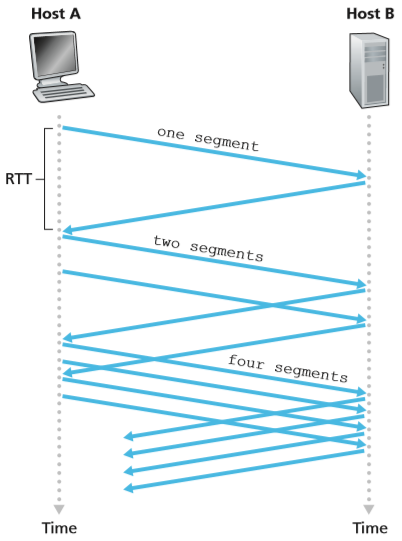
\includegraphics[width=0.35\textwidth]{TCP_Slow_Start}
%     \captionsetup{width=0.35\textwidth}
%     \caption{\gls{tcp} slow start.}
% \end{wrapfigure}

% With the initial \gls{cwnd} size set, say $1$ \gls{mss} for simplicity sake, the goal of the slow start phase is simple; find the amount of available bandwidth, \textit{quickly}.

% To do this, \gls{tcp} will first send one segment of size $1$ \gls{mss} into the network, and for every \gls{ack}, increase 

Slow start and congestion avoidance are two independent algorithms with
different objectives, but in practice are implemented together and so will be discussed together.

Upon a \gls{tcp} connection, the \gls{cwnd} value is initialized to a single \textit{segment} with a specified size. This size is either  announced by the the other end, known as the \gls{rwnd}, or set to a typical default \cite{rfc5681}. In the same sense that \gls{cwnd} is a sender-side limit, \gls{rwnd} is a receiver-side limit. Together, the minimum of \gls{cwnd} and \gls{rwnd} governs the data transmission in slow start. However, at the beginning of a transmission, the network conditions are unknown, so the goal of the slow start phase is simple; slowly probe the network to determine the available capacity.

To find the capacity, slow start works as follows; the sender starts by transmitting one segment. For every received \gls{ack}, increment the \gls{cwnd} by another segment, effectively doubling it every \gls{rtt}. Repeat this process until a timeout occurs. That is, until the capacity has been reached that is signaled by a router starting to drop packets, which tells the sender that its \gls{cwnd} has grown too large.

\begin{figure}[H]
    \centering
    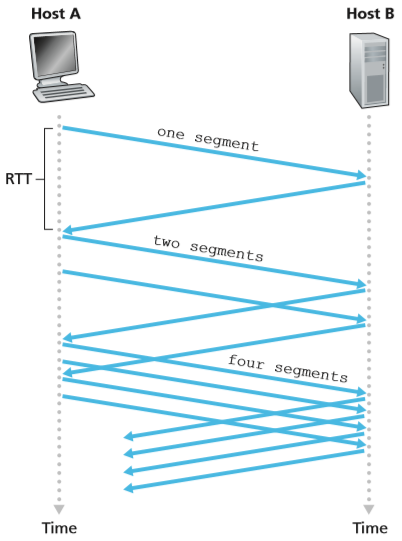
\includegraphics[width=0.4\textwidth]{TCP_Slow_Start}
    \captionsetup{width=0.4\textwidth}
    \caption{\gls{tcp} slow start. Despite the name, the sending rate experiences exponential growth. \todo{update image}}
\end{figure}

As a response to hitting the threshold, \gls{tcp} will now halve the \gls{cwnd} since that is the last known value to not induce a timeout. This new value is known as the \gls{ssthresh}, and is another \gls{tcp} state variable used to determine whether the slow start or congestion avoidance algorithm is used to control the data transmission. In other words, the slow start phase ends when \gls{cwnd} reaches or exceeds \gls{ssthresh}.

The goal of congestion avoidance is also simple; avoid congestion, as the name implies. But the challenge here is to maintain a transmission rate that it not too low, otherwise the link becomes underutilized, and at the same time probe for available bandwidth without overflowing the network too quickly. To do so, a feedback control algorithm known as \gls{aimd} is used. \gls{aimd} provides linear growth of the \gls{cwnd} when probing for available bandwidth, and a multiplicative reduction when congestion is detected.

\begin{figure}[H]
    \centering
    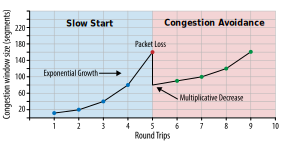
\includegraphics[width=0.7\textwidth]{TCP_Congestion_Control_Simple}
    \captionsetup{width=0.7\textwidth}
    \caption{The two main parts of \gls{cc}; the slow start phase where \gls{cwnd} grows exponentially, and the congestion avoidance phase where the transmission rate is increased more conservatively. (\href{https://hpbn.co/building-blocks-of-tcp/}{\textit{source}})}
\end{figure}

\todo{maybe write more about AIMD with some math}
\todo{addd conclusion to this section}


\subsubsection{Fast Retransmit and Fast Recovery}

Every packet sent using TCP has a \textit{sequence number}, so that the data can reassembled in correct order on the receiver side. But it is important to note that \gls{tcp} may send an out-of-order packet, to which the receiver should act upon immediately by sending back a duplicate \gls{ack}.

\todo{follow up...}



% \subsubsection{Congestion Avoidance}
% \subsubsection{Fast Retransmit}
% \subsubsection{Fast Recovery}




% The answer is simple; \textit{start slow}. First, set the \gls{cwnd} to a small multiple of the \gls{mss} allowed on the \gls{tcp} connection. Then, start probing for available bandwidth. For every received \gls{ack}, double the \gls{cwnd} until a timeout occurs. This phase is known as the \textit{slow start}, which lasts until \gls{cwnd} reaches the threshold value, known as the \gls{ssthresh}, and is signaled by a timeout.

% With the threshold hit, \gls{tcp} now has an idea of the maximum amount of data it can transmit, and therefore sets the \gls{cwnd} value to half of the \gls{ssthresh} value since that is the last known value to not induce a timeout. From this point, the \textit{congestion avoidance} phase starts. Here, the \gls{cwnd} value is additively increased by one \gls{mss} every \gls{rtt}.





% \begin{figure}[H]
%     \centering
%     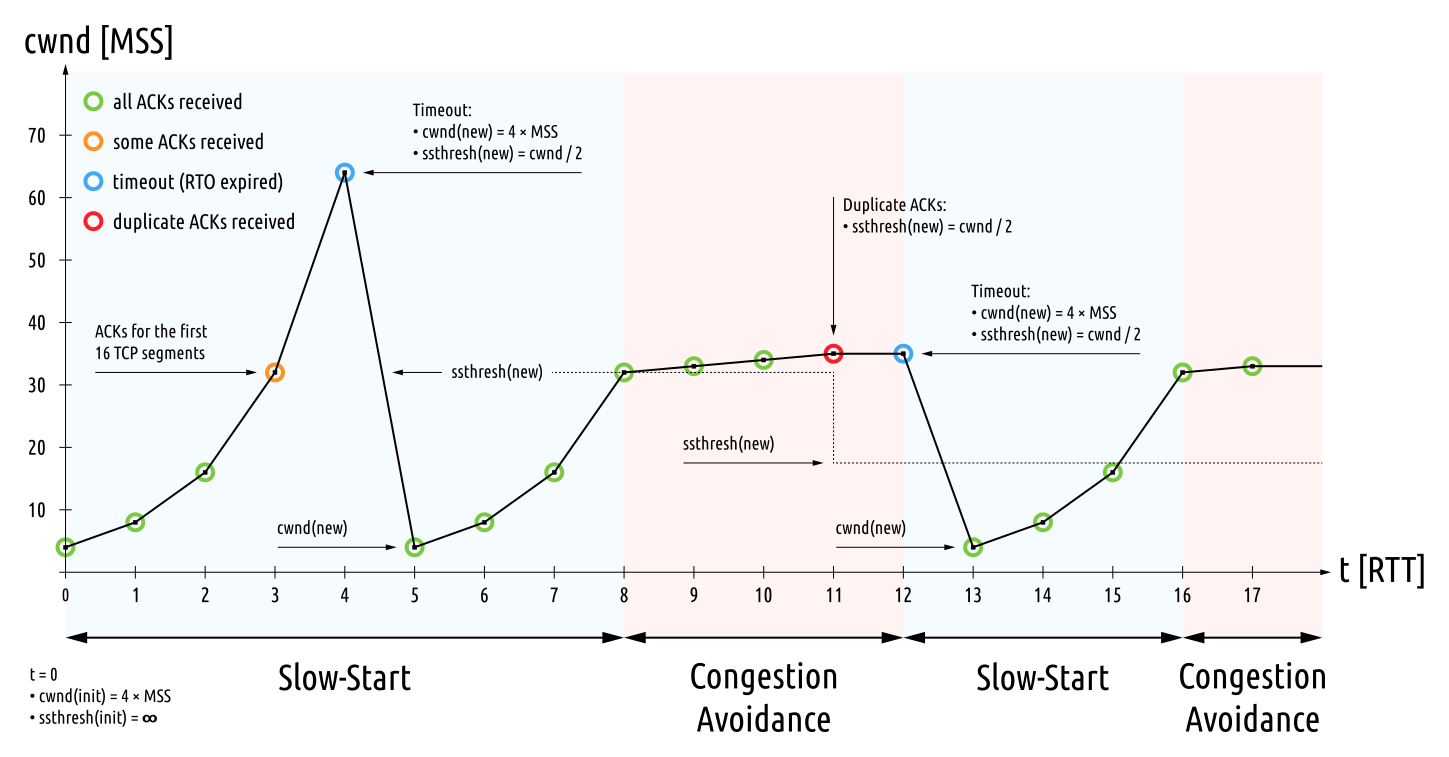
\includegraphics[width=1.0\textwidth]{TCP_Slow-Start_and_Congestion_Avoidance}
%     \captionsetup{width=0.95\textwidth}
%     \caption{Example of ioj oij io iojio joiojioj iojio joi jio joi jioj ioj io jio jioj ioj io jio ijojiojoijoij a parametric plot ($\sin (x), \cos(x), x$)}
% \end{figure}



% To help reduce congestion on the links \gls{tcp} maintains a \gls{cwnd}, which limits the total number of unacknowledged packets that it can send at a time. This is done in multiple fases.

% In the slow start fase,  right after a connection is established. the congestion window starts as a small multiple of \gls{mss} and is effectively doubled for every \gls{rtt}. When it reaches the slow-start threshold(ssthresh), \gls{cwnd} is reduced by half and a new fase starts, congestion avoidance. In this fase \gls{cwnd} is increased linearly by one \gls{mss} every \gls{rtt}. If loss occurs, it could mean there is congestion, and steps will be taken to reduce load on the network. The steps depend on what exact congestion avoidance algorithm is used.

\subsection{TCP Tahoe and Reno}

\todo{show some early examples TCP congestion-control algorithms}

\begin{figure}[H]
    \centering
    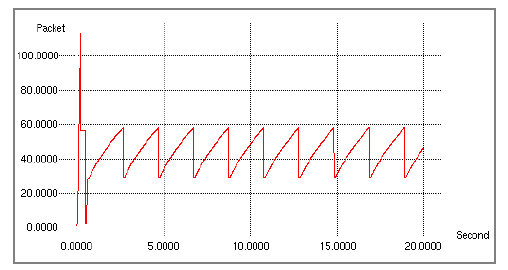
\includegraphics[width=0.6\textwidth]{TCP_CC_NewReno}
    \captionsetup{width=0.6\textwidth}
    \caption{The classic \textit{sawtooth} pattern of \gls{cwnd} using an older \gls{tcp} congestion-algorithm known as \textit{NewReno}. \todo{update image}}
\end{figure}





\section{Active Queue Management}



\section{Explicit Congestion Notification}

\gls{ecn} is an extension to TCP that allows routers to notify end points on impending congestion \textit{without} dropping packets.

\subsection{Legacy ECN}

In legacy ECN, the router notifies end hosts of congestion by setting a Congestion Encountered (CE) flag in the IP header on ECN enabled packets when experiencing congestion. The reciever of the packet then reflects this back to the sender by setting an ECN-Echo (ECE) in the TCP header. It keeps doing this until the sender responds back with a segment with Congestion Window Reduced (CWR) set, indicating that the sender has backed off.

\subsection{Accuracy ECN}

\section{Alternative Backoff with ECN}

